% !TEX root = ThesisGchatzi.tex

\section{Computing Tile Map Summaries}
\label{sec:tilemap_summary}

\graphicspath{{Papers/ElsevierBigDataResearch/}}

In the following, we present our second visualization method, which allows the user to draw one or more timeboxes on the time series domain. This triggers a traversal of our hybrid \hisax index to obtain the geolocated time series in the currently visible map area and also fully contained within these timeboxes. The result comes in the form of tiles, each spanning between two \isax breakpoints, along with a count per tile indicating the number of time series whose SAX symbol resides within that tile. This count is used to generate the visualization in the form of tile map. A predefined number of MBRs and corresponding counts is also returned, generated by clustering the locations of the resulting geolocated time series and used for the spatial part of the visualization. Whenever the user zooms in/out or pans over the map, or whenever she draws a new timebox, the procedure is repeated, the index is traversed and the visualization is regenerated. Next, we first outline the original structure of the \isax index and then we introduce its \hisax variant, which enables evaluation of timebox queries and also maintenance of spatial information in its nodes. As we discuss next, those two extensions provide the necessary support for computing tile map summaries as specified in Section~\ref{subsec:tilemap_sums}.

\begin{figure}[!t]
 \centering
 \subfloat[Sample dataset with MBRs as maintained by \hisax.]{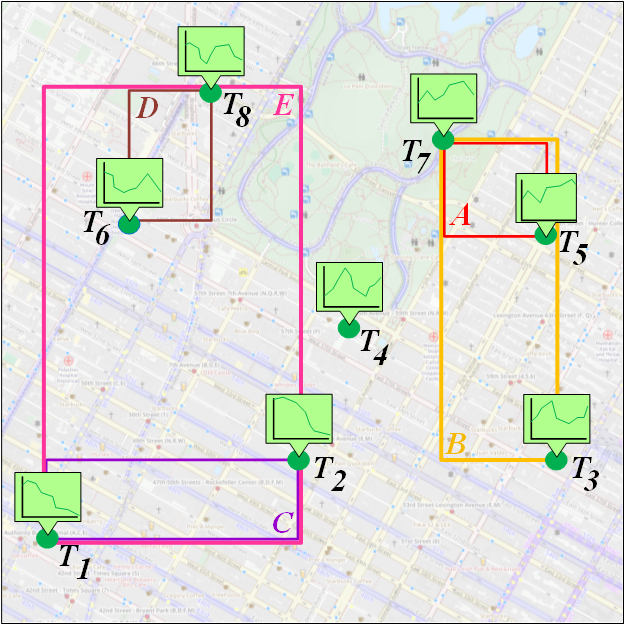
\includegraphics[width=70mm]{figures/geoISAX_mbr.png}\label{subfig:sample}} \\
 \subfloat[The \hisax index with letters indicating MBRs (depicted in \ref{subfig:sample}) attached to each node. Nodes with filled boxes indicate a degenerate MBR consisting of a single point; nodes with hollow  boxes indicate no data. Subtrees under dash lines are not shown for brevity.]{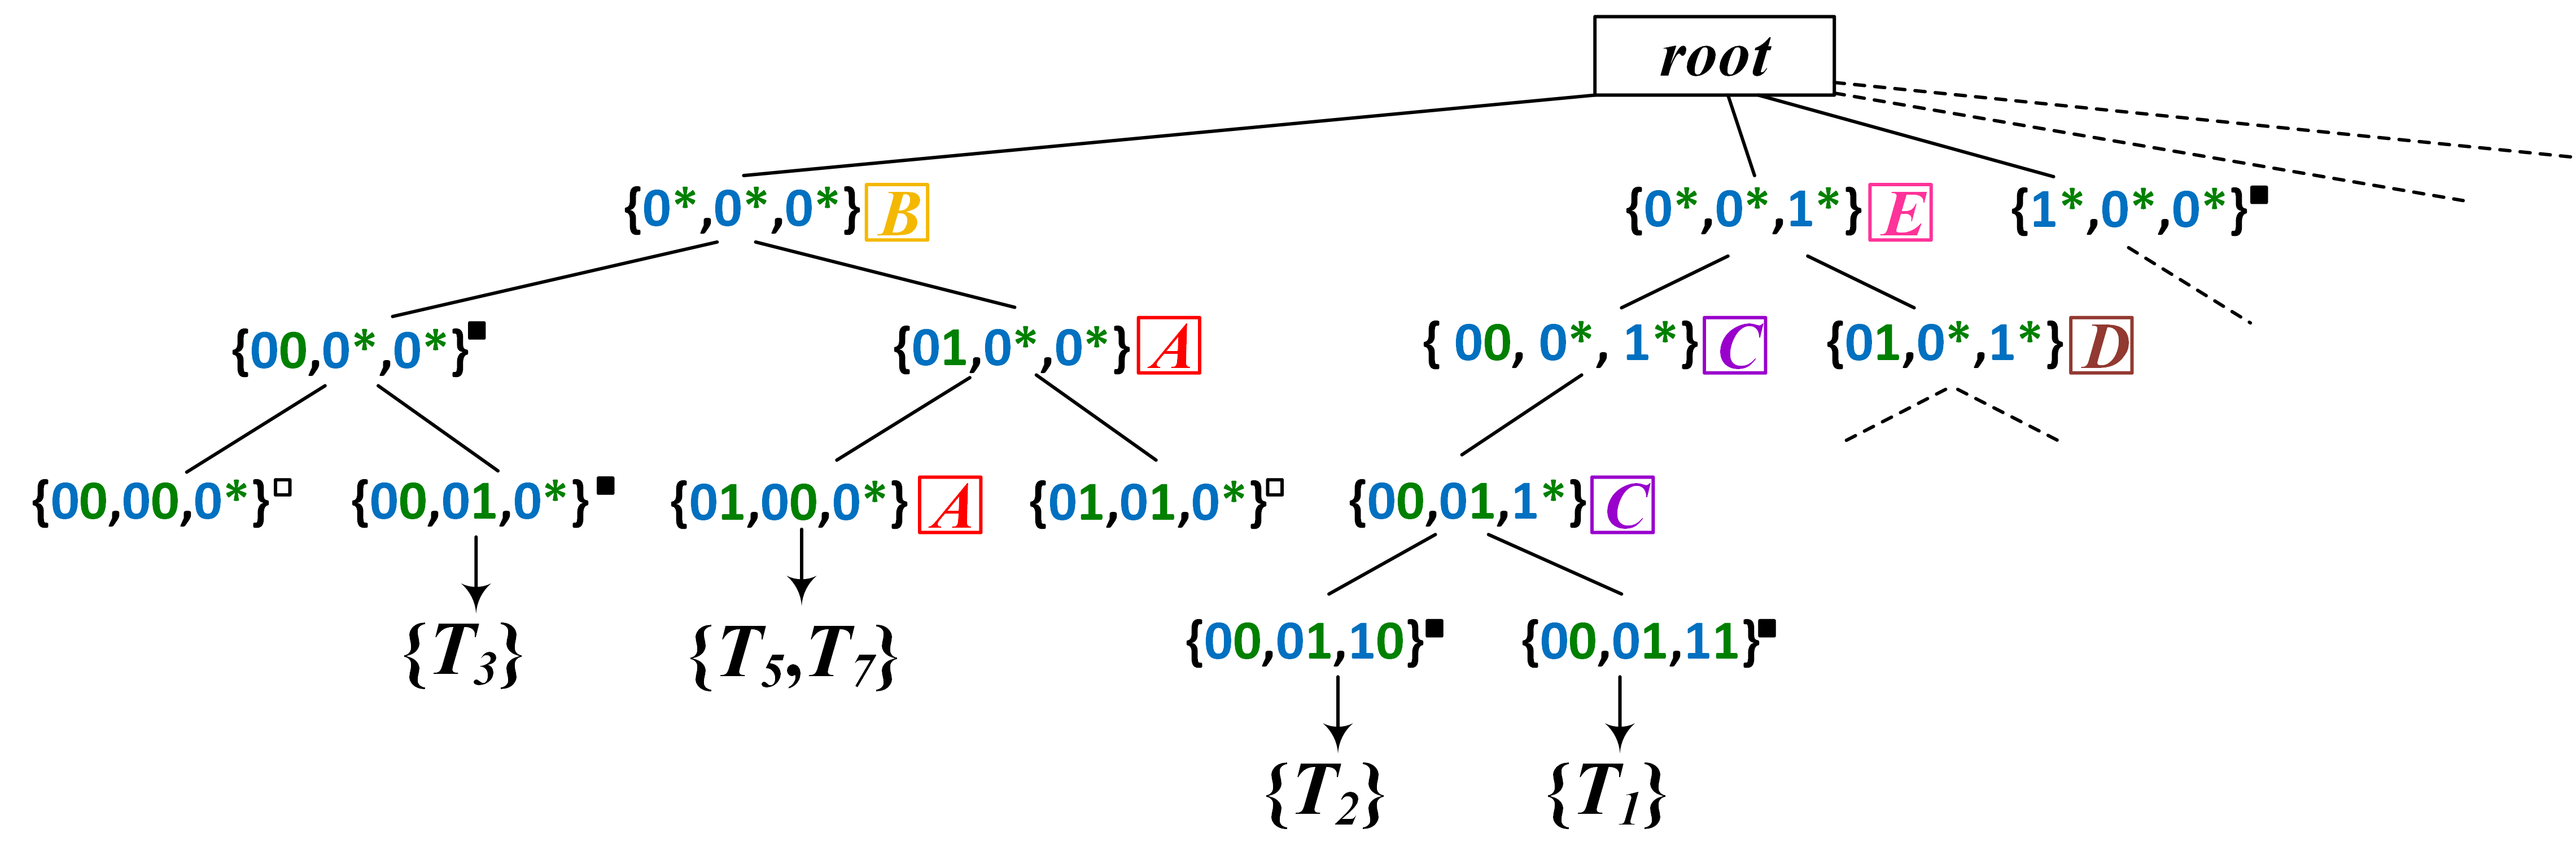
\includegraphics[width=0.99\textwidth]{figures/isax_tree2.png}\label{subfig:isaxtree}}
 \caption{Sample dataset with MBRs and SAX representations of time series as maintained by the \hisax index.}
 \label{fig:example}
\end{figure}

\subsection{The \hisax Index}
\label{subsec:hisax}

We introduce \hisax, a time series-first {\em hybrid} variant of the \isax index that allows significant traversing speed-ups by pruning both on the spatial and time series domain. This is achieved by storing in each node of the tree, apart from the SAX word of the geolocated time series it contains, the MBR that they form. Initially, the time series part of the index is built, following the procedure described in Section~\ref{sec:ts_index_query_explore}. As a next step, similarly to the \btsr index, we traverse the index in a bottom-up fashion, first generating the MBRs of the geolocated time series contained in the leaf nodes. As we go upwards, we update the MBR information of each visited inner node, using the MBRs of its children nodes, until we reach the root, whose MBR will contain the geolocated time series of the whole dataset. Figure~\ref{subfig:isaxtree} illustrates the structure of the \hisax tree created over a sample dataset of geolocated time series.

Due to the fact that the \isax index is created to solely index time series data, the MBRs generated by our hybrid variant may be highly overlapping, mitigating the pruning potential while traversing the index. To alleviate the negative effects of the numerous overlaps, we introduce an alternative {\em splitting policy} for \hisax, which attempts to minimize the overlapping area, while maintaining the total area covered by the MBRs that occur after a split at the lowest possible levels. Recall that the original \isax index selects the split dimension (i.e., the segment of a node's word on which the split will occur) for a node using a round robin approach. Our method loops over all split dimensions and for each one, it calculates the SAX word that would occur upon splitting on it. Then, it generates the MBRs for that specific split using the location of the geolocated time series contained in the node to be split. For each split dimension, it computes the sum of the two new MBRs' intersection area and the total area that they cover. The selected split is the one that generates the smaller sum. Due to the rather small number of word segments in an \isax index, this procedure does not incur high construction costs, only slightly affecting the overall index construction time.

\subsection{Deriving Tile Map Summaries from the \hisax Index}
\label{subsec:tilemapvis}

Next, we present our summarization approach for tile map visualization of geolocated time series, obtained using timeboxes. In order to maintain low latency even for large datasets, we traverse \hisax to obtain the resulting geolocated time series in a timely fashion. However, to avoid false negatives, we need to ensure that the pruned nodes do not contain any qualifying geolocated time series, as we discuss next. 

\begin{figure}[!t]
 \centering
 \subfloat[Outside below]{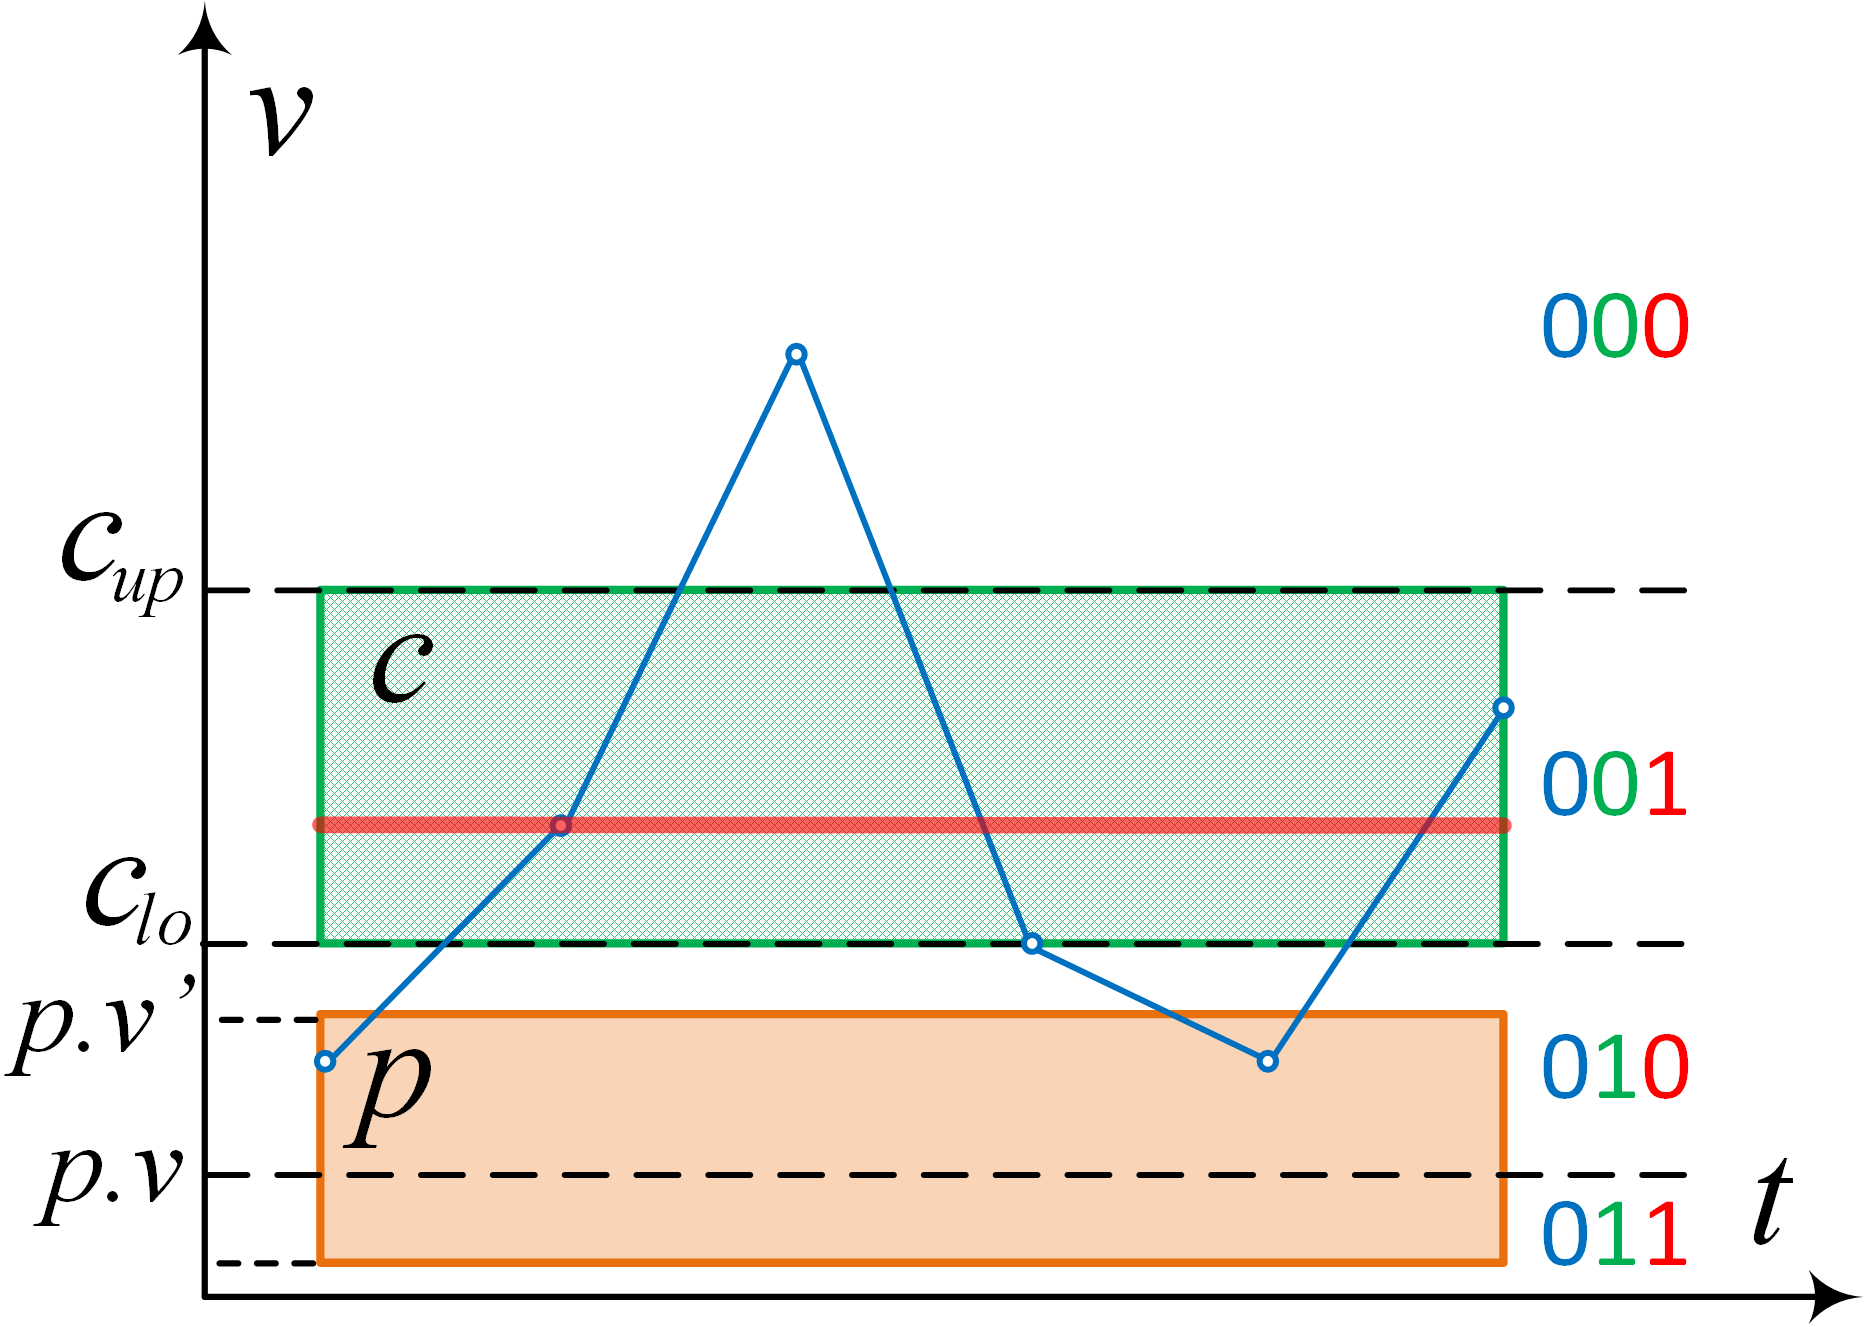
\includegraphics[width=0.24\textwidth]{figures/breakpoints1.png}\label{subfig:breakpoints1}}
 \subfloat[Outside above]{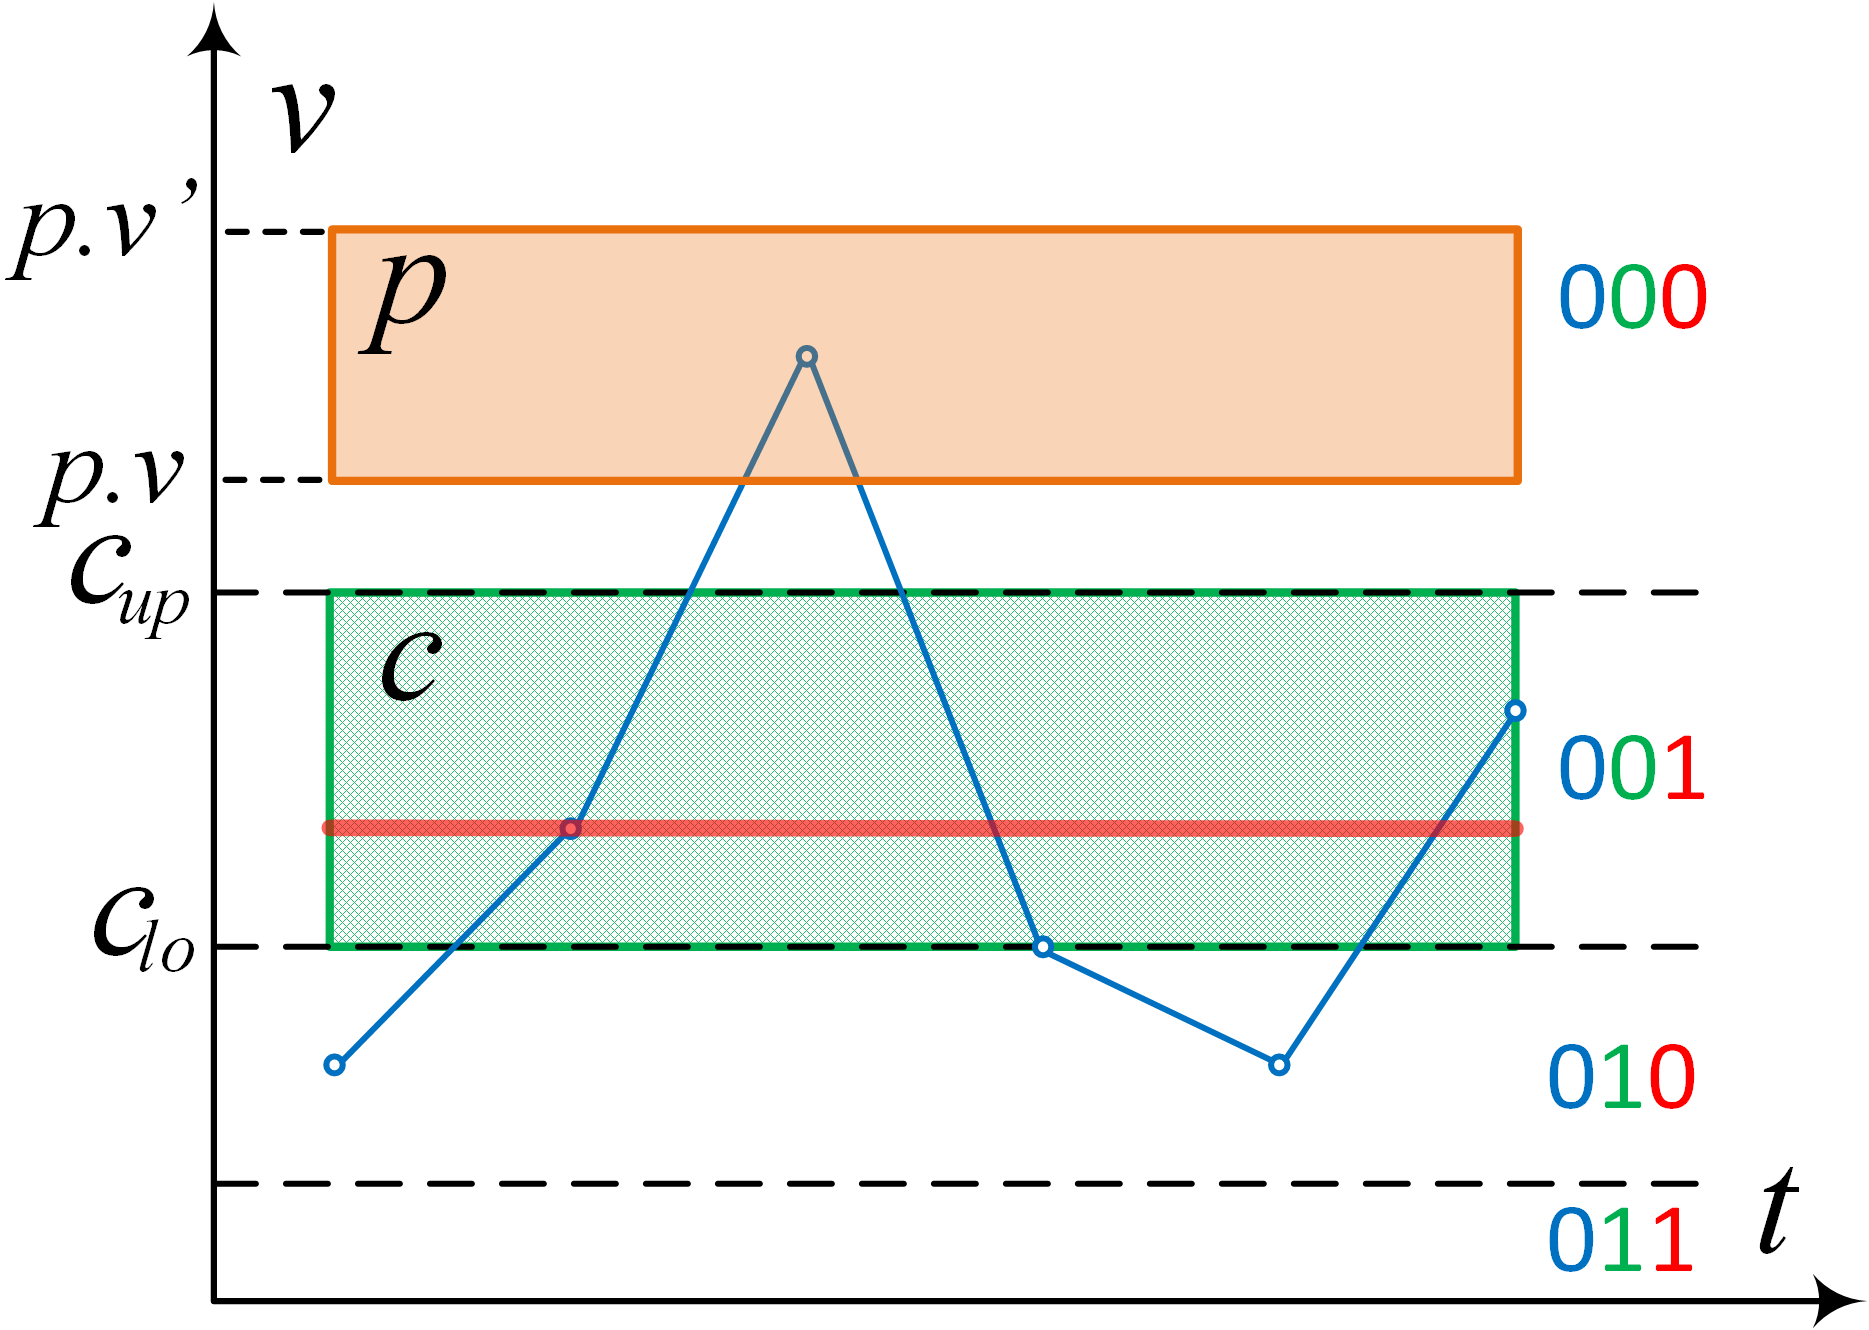
\includegraphics[width=0.24\textwidth]{figures/breakpoints2.png}\label{subfig:breakpoints2}}
 \subfloat[Intersecting below]{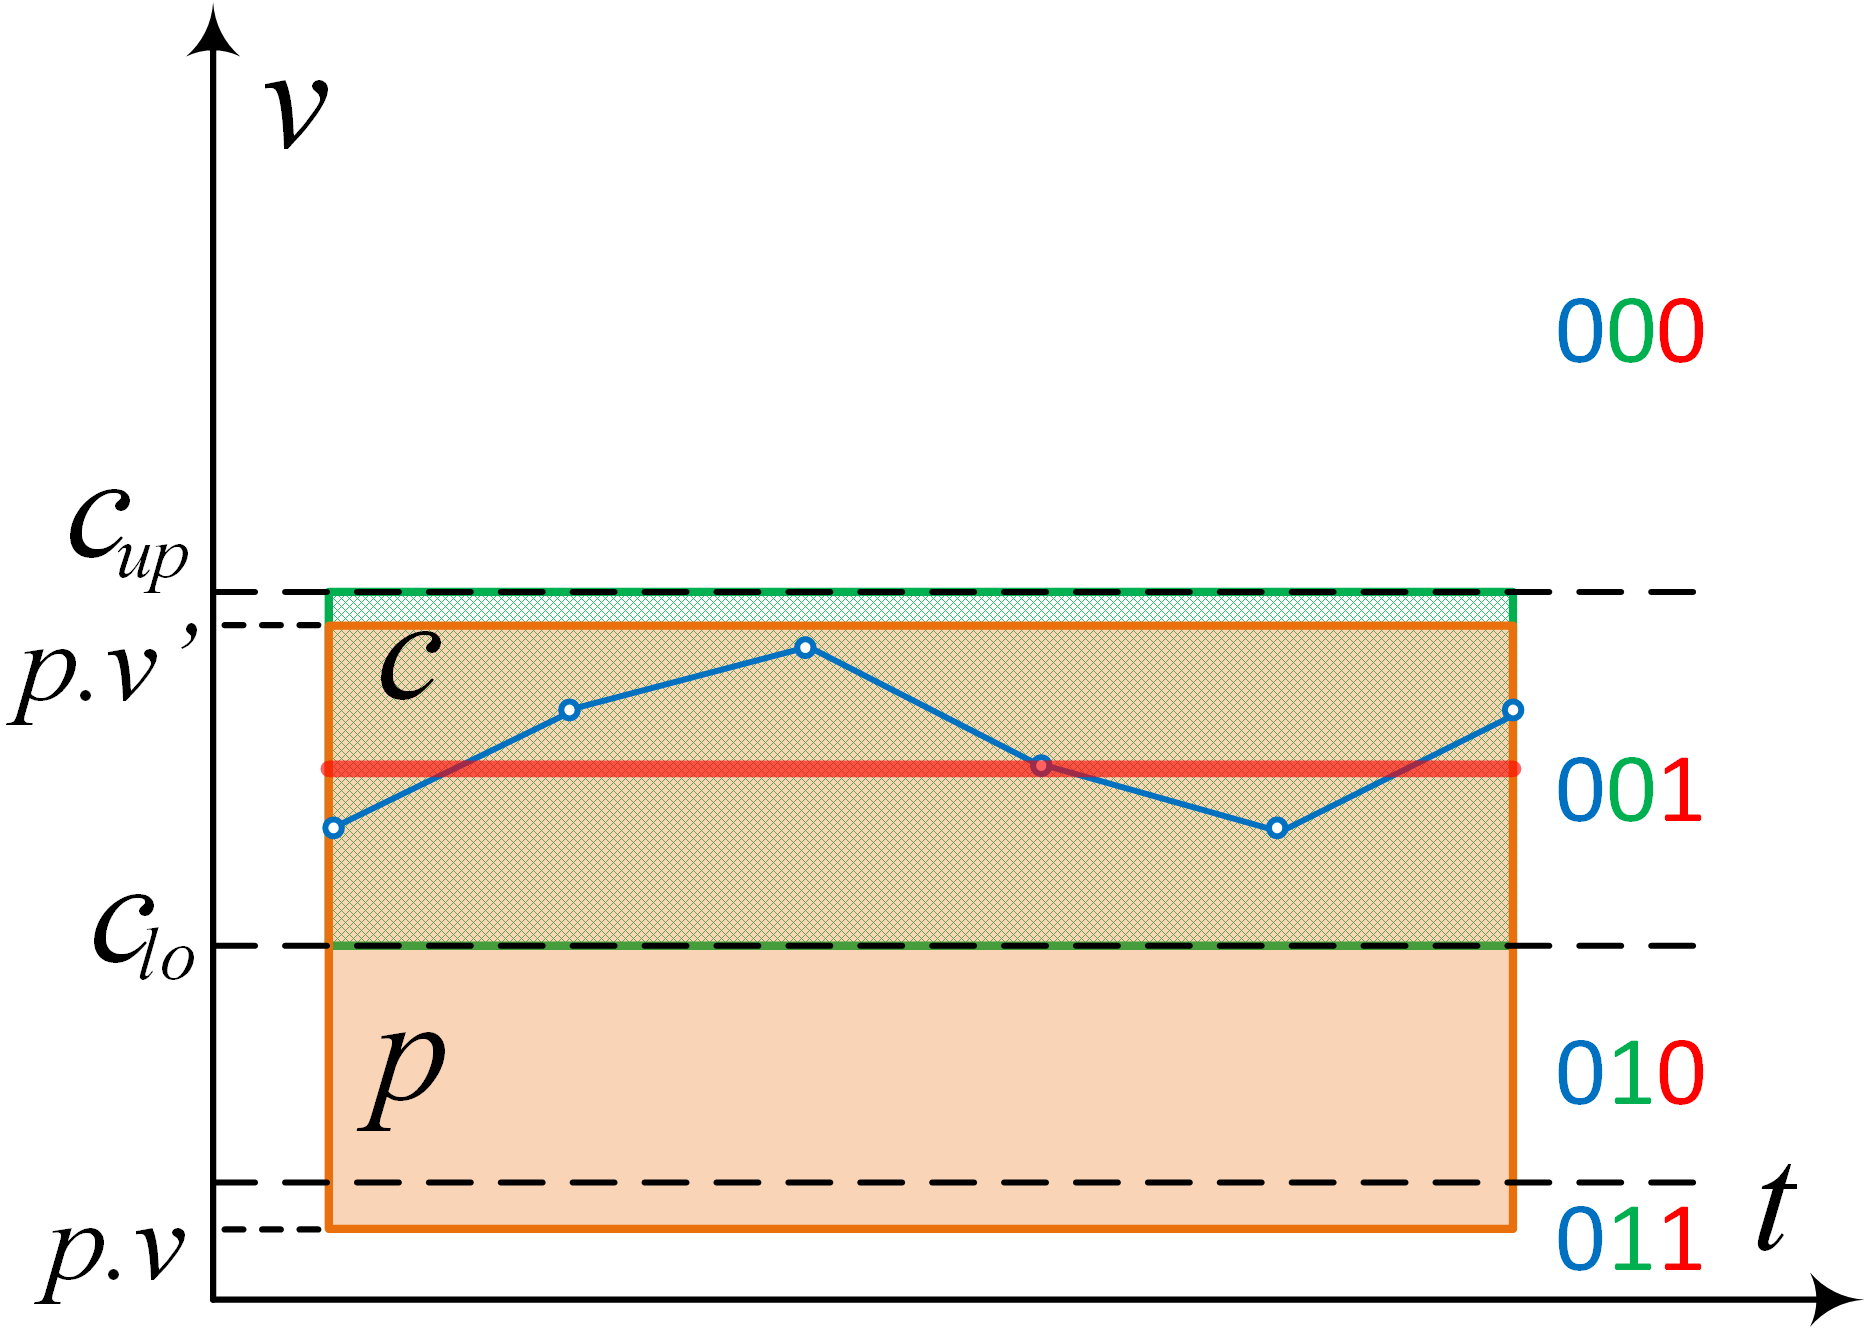
\includegraphics[width=0.24\textwidth]{figures/breakpoints4.png}\label{subfig:breakpoints3}}
 \subfloat[Intersecting above]{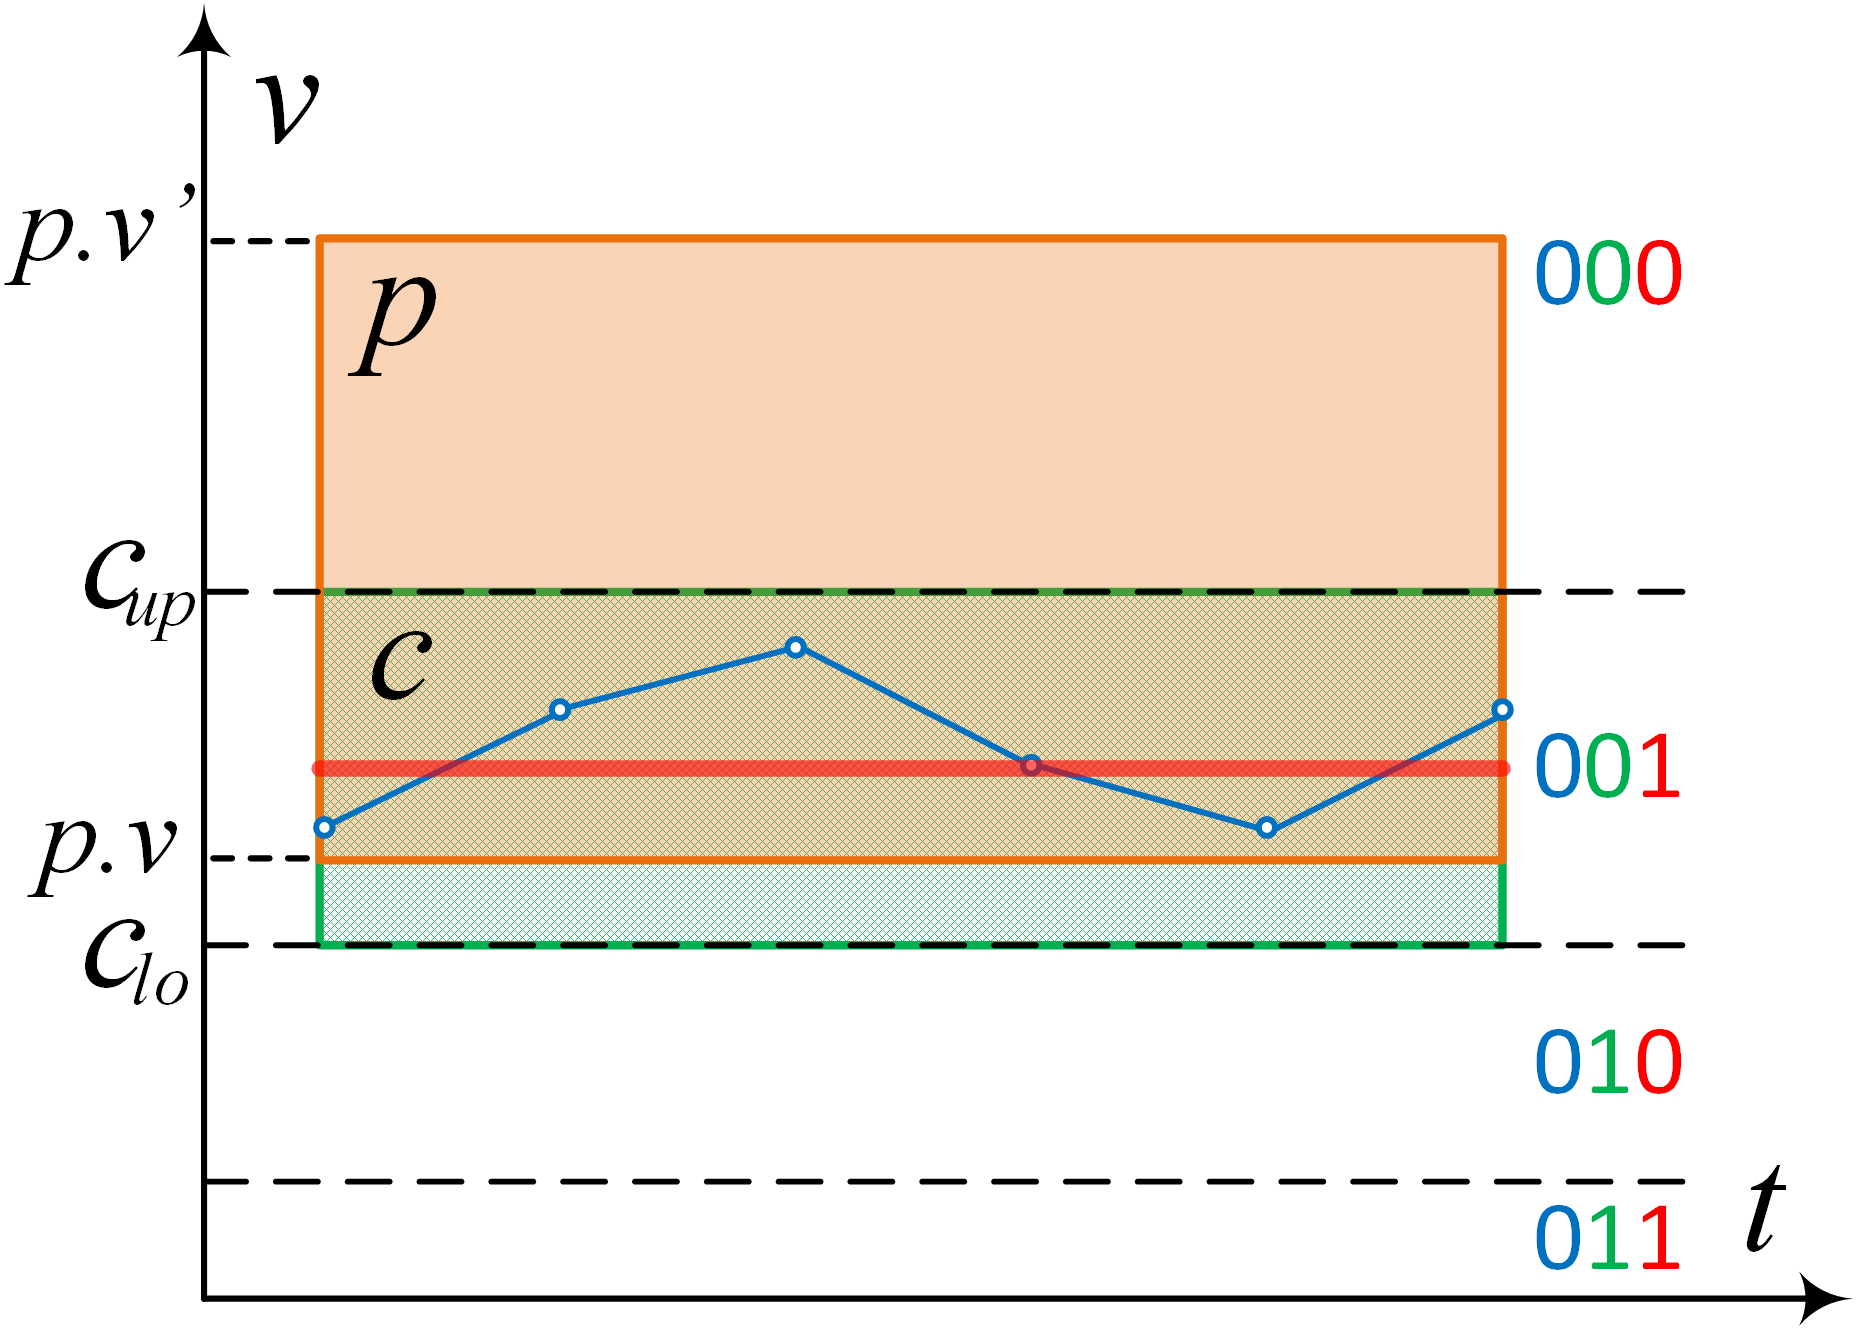
\includegraphics[width=0.24\textwidth]{figures/breakpoints3.png}\label{subfig:breakpoints4}}\
\caption{Cases where a timebox $p$ is either outside or intersecting a given tile $c$.}
\label{fig:br_outside}
\end{figure}

\emph{Pruning Rule for Timebox Queries on \hisax.}
When traversing the \hisax index, we first evaluate whether its MBR satisfies the spatial constraint $q$ (i.e., intersects with or is within $q$). If so, we need to check the timebox constraint $p$, i.e., whether the time series it contains {\em certainly} have data points that reside outside the given timebox. Consider the time series in Figure~\ref{fig:br_outside}. Without loss of generality, we suppose a SAX word of length $w=1$ and cardinality $b=8$, i.e., $SAX(T,1,8)=\{010\}$. The solid red horizontal line is the PAA value that classifies this segment of the time series to the SAX value $010$. Tile $c$ defined by the two breakpoints that contain the PAA value is hown in green color, while the user-defined timebox $p$ specifying a value range $[v,v')$ is depicted in orange.

As can be noticed in Figure~\ref{subfig:breakpoints1}, the upper side of the timebox is below the lower side of tile $c$, i.e., $p.v'<c_{lo}$. In this case, we can safely prune a node that is described by this SAX word, because there is at least one data point outside the timebox, ``pulling'' the PAA upwards and within $c$. For the same reasons, we can prune a node whose breakpoint-defined area is completely below the given timebox, as depicted in Figure~\ref{subfig:breakpoints2}. In this case, the lower side of the timebox is above the upper side of $c$ ($p.v>c_{up}$), indicating that there is at least one data point outside the timebox ``pulling'' the PAA value downwards and within $c$.

\begin{algorithm}[ht!]
  \DontPrintSemicolon
  \KwIn{The input rectangle $q$; the timebox $p$; the number of MBRs to be generated $k$}
  \KwOut{A list $R_t$ containing a tile map and tuples of MBRs and object counts}
  \vspace{6pt}
  $R_t \leftarrow IndexTraversal(Root, q, p, k)$ \\
  \KwRet $R_t$ \\
  \vspace{6pt}
  \SetKwProg{procTraversal}{Procedure}{}{}
  \procTraversal{$IndexTraversal(Root, q, p, k)$}{
    $R_t \leftarrow \emptyset, R \leftarrow \emptyset, tmap \leftarrow \emptyset, L \leftarrow \emptyset, Q \leftarrow Root.getChildren()$ \\
    \While{$Q \neq \emptyset$}{
      $N \leftarrow Q.getNext()$ \\
      \If{$N$ is not leaf}{
        \ForEach{$N' \in N.getChildren()$}{
          \If{$q.contains(N'.mbr) \lor q.overlaps(N'.mbr)$}{
            \If{$timebox(N'.sax, p)$}{
              $Q \leftarrow Q \cup N'.getChildren()$ \\
            }
          }
        }
      }
      \Else {
        \ForEach{$T \in N'.getChildren()$}{
          \If{$timebox(T, p$)}{
            $tmap \leftarrow updateCounts(tmap, T.sax)$ \\
            $R \leftarrow R \cup T$ \\
          }
        }
        $L \leftarrow L \cup \{R.mbr, |R| \}$ \\
      }
    }
    $\{ \langle mbr, cnt \rangle \} \leftarrow kmeans(L, k)$ \\
    $R_t \leftarrow \{\langle tmap, \{ \langle mbr, cnt \rangle \} \rangle \}$ \\
    \KwRet $R_t$ \\
  }
  \vspace{6pt}
  \SetKwProg{procTimeboxCheck}{Procedure}{}{}
  \procTimeboxCheck{$timebox(X, p)$}{
    \If{$isSax(X)$}{
      \ForEach{$s \in \{p.t_{min}, p.t_{max}\}$}{
        $c \leftarrow breakpoints(X_s)$ \\
        \If{$p.v_{min} > c_{up} \lor p.v_{max} < c_{lo}$}{
          \KwRet $False$ \\
        }
      }
      \KwRet $True$ \\
    }
    \Else{
      \ForEach{$t \in \{p.t_{min}, p.t_{max}\}$}{
        \If{$X_t > p.v_{max} \lor X_t < p.v_{min}$}{
          \KwRet $False$ \\
        }
      }
      \KwRet $True$ \\
    }
  }
  \caption{Tile Map Summarization of Geolocated Time Series}
  \label{alg:algorithm2}
\end{algorithm}

On the other hand, in case the timebox intersects with tile $c$, we cannot safely prune the corresponding node. For example, in Figure~\ref{subfig:breakpoints3}, $c_{lo} < p.v' < c_{up}$, so there may exist a time series that is fully contained in the timebox and thus be part of the result. The same stands for the example in Figure~\ref{subfig:breakpoints4}, where  $c_{lo} < p.v < c_{up}$. Finally, for the cases where timebox $p$ fully contains tile $c$ or vise-versa, it is trivially deduced that no pruning can apply.

We stress that the above observations only hold when in the time axis the given timebox is aligned to the segments of the SAX words in the index. For example, for a time series of length $n=10$ and a word length of $w=5$, the resulting segments will have length equal to $n/w=2$. Thus, the timebox must be aligned to the data points $t_0, t_2, t_4, t_6$ and $t_8$.

\emph{Traversal Algorithm over \hisax.} Algorithm~\ref{alg:algorithm2} outlines the process for producing the tile map visualizations of geolocated time series. The process takes as input a spatial rectangle $q$, a user-defined timebox $p$ and the number $k$ of MBRs that will be returned. It produces a list $R_t$ containing $k$ tuples of MBRs along with time series counts and the tile map, as defined in Eq.~\ref{eq:bundles_sum}. For each inner node, the procedure checks whether its MBR intersects rectangle $q$ and whether its SAX word might represent time series within timebox $p$. If a leaf node is reached and both constraints are met, we iterate over its raw geolocated time series and add the ones qualifying for the timebox to the final result $R_t$, after properly updating the breakpoint tile counts.

In more detail, the procedure takes place as follows. Starting from the root of the \hisax index, we iterate over each node's children (Lines 5-6 in Algorithm~\ref{alg:algorithm2}). Next, we check whether the node to be evaluated is a leaf node (Line 8) and if it is not, we iterate over its children (Line 9) and check whether each one's MBR either is contained or intersects the spatial rectangle (Line 10). If so, we check whether its SAX word could represent time series within the timebox (Line 11) and if this is the case, we add it to the queue $Q$ to be evaluated (Line 12). At this point, we should mention that, in order to avoid expensive calculations, we first perform the spatial check as it is less computationally expensive than the timebox check, avoiding the latter in case the node's MBR is outside the input rectangle. If the currently evaluated node is a leaf node (Line 13), we iterate over the geolocated time series that it contains (Line 14) and check whether it is fully contained within the user-defined timebox (Line 15). If so, we update the tile counts matrix $tmap$ (Line 16) and add the corresponding raw time series to the set $R$ (Line 17). Finally, we add to a list $L$ the MBR of the set of qualifying time series along with its size (Line 18). Upon exiting the loop, we apply $k$-means clustering on the resulting centroids and obtain $k$ tuples containing MBRs along with time series counts. 

The procedure that checks whether a SAX word could represent time series that are fully contained within the given timebox is described in detail starting from Line 22 in Algorithm~\ref{alg:algorithm2}. It takes as input a timebox and a raw time series or SAX word that we want to check against the given timebox. We initially check whether the given $X$ argument is a SAX word (Line 23). If it is, we itereate over all the segments that are contained (Line 22) in the time range defined by the timebox and for each segment we obtain the \isax breakpoints that enclose it (Line 25). Afterwards, we check whether the lower side of the timebox is above the upper side of the tile defined by the obtained breakpoints, or vice versa, as depicted in Figure~\ref{fig:br_outside}. If this is true, we return false. If this is not the case for any of the segments, the method returns true (Line 28). A similar procedure is followed for the case that argument $X$ is a raw time series (Lines 29-33).